% THIS IS SIGPROC-SP.TEX - VERSION 3.1
% WORKS WITH V3.2SP OF ACM_PROC_ARTICLE-SP.CLS
% APRIL 2009
%
% It is an example file showing how to use the 'acm_proc_article-sp.cls' V3.2SP
% LaTeX2e document class file for Conference Proceedings submissions.
% ----------------------------------------------------------------------------------------------------------------
% This .tex file (and associated .cls V3.2SP) *DOES NOT* produce:
%       1) The Permission Statement
%       2) The Conference (location) Info information
%       3) The Copyright Line with ACM data
%       4) Page numbering
% ---------------------------------------------------------------------------------------------------------------
% It is an example which *does* use the .bib file (from which the .bbl file
% is produced).
% REMEMBER HOWEVER: After having produced the .bbl file,
% and prior to final submission,
% you need to 'insert'  your .bbl file into your source .tex file so as to provide
% ONE 'self-contained' source file.
%
% Questions regarding SIGS should be sent to
% Adrienne Griscti ---> griscti@acm.org
%
% Questions/suggestions regarding the guidelines, .tex and .cls files, etc. to
% Gerald Murray ---> murray@hq.acm.org
%
% For tracking purposes - this is V3.1SP - APRIL 2009

\documentclass{acm_proc_article-sp}
\usepackage{url}
\begin{document}

\title{Exploring Music Review Score Prediction (2012)}

%
% You need the command \numberofauthors to handle the 'placement
% and alignment' of the authors beneath the title.
%
% For aesthetic reasons, we recommend 'three authors at a time'
% i.e. three 'name/affiliation blocks' be placed beneath the title.
%
% NOTE: You are NOT restricted in how many 'rows' of
% "name/affiliations" may appear. We just ask that you restrict
% the number of 'columns' to three.
%
% Because of the available 'opening page real-estate'
% we ask you to refrain from putting more than six authors
% (two rows with three columns) beneath the article title.
% More than six makes the first-page appear very cluttered indeed.
%
% Use the \alignauthor commands to handle the names
% and affiliations for an 'aesthetic maximum' of six authors.
% Add names, affiliations, addresses for
% the seventh etc. author(s) as the argument for the
% \additionalauthors command.
% These 'additional authors' will be output/set for you
% without further effort on your part as the last section in
% the body of your article BEFORE References or any Appendices.

\numberofauthors{1} %  in this sample file, there are a *total*
% of EIGHT authors. SIX appear on the 'first-page' (for formatting
% reasons) and the remaining two appear in the \additionalauthors section.
%
\author{
% You can go ahead and credit any number of authors here,
% e.g. one 'row of three' or two rows (consisting of one row of three
% and a second row of one, two or three).
%
% The command \alignauthor (no curly braces needed) should
% precede each author name, affiliation/snail-mail address and
% e-mail address. Additionally, tag each line of
% affiliation/address with \affaddr, and tag the
% e-mail address with \email.
%
% 1st. author
\alignauthor
Patrick Marchwiak\\
       \email{pd@marchwiak.com}
}

\maketitle
\begin{abstract}
Much of the popular and independent music released today is critically
reviewed and judged on its quality and artistic merit.
This is typically considered a subjective art performed by a human.
This paper seeks to explore how well a computer can predict the
general quality of a piece of music using music information retrieval and
data mining techniques.
\end{abstract}

\section{Data Gathering and Integration}
Manipulation of data and metadata needed to be repeated multiple times
and with various parameters thus a modular pipeline architecture was used where
the output of the previous process or script was used as the input to the 
next. In steps where data was acquired from an external source, it was
saved to disk and processed from disk by the next step rather than in memory
to minimise the amount of communication needed with the external sources.

Metacritic.com was used as the starting point for all data. Metacritic is a
review aggregation website which normalizes scored reviews (those assigned
a letter grade or numeric score in some range) to their own 0-100 scale
and assigns scores to reviews without scores based on their overall sentiment.
This methodoloy is somewhat controversial as it reduces
all reviews to a single score losing all of the rich descriptive textual
information. However this type of data works very well in the context
of machine learning since reasoning about a ``metascore'' is simpler
as well as gets closer to the notion of an objective measure of quality for an album.

\setlength\fboxsep{0pt}
\setlength\fboxrule{0.5pt}
\fbox{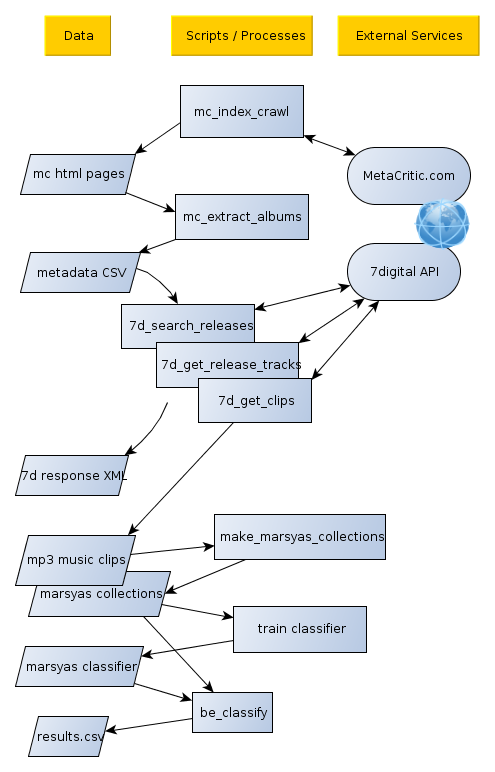
\includegraphics[scale=0.45]{pipeline-diagram}}
\\
Figure 1: Metadata and audio processing pipeline\\




The Metacritic website displays
reviews grouped by genre and sorted by date. These index pages were downloaded
as HTML. The next script parsed out artist, album, and metascores and wrote them
to a flat file (CSV). 

A number of approaches were considered for acquisition of music files.
Firstly, the use of personal music libraries was evaluated. These were
found to be unsatisfactory as the overlap between them and the data on metacritic
was not substantial. Additionally, people naturally tended to own more music
that was rated highly which would result in an unbalanced sample set.

The second approach considered and the one ultimately used was the 7digital API
service. 7digital is primarily a digital media distribution company
and their API provides access to a wide range of metadata from their music catalog.
With artist and album names in hand, these were used as input into another script
which searched for releases with those names using the ``release/search'' resource.
For each matching release, a track list was obtained using the ``release/tracks'' resource.
The obtained track ids were finally used to obtain 30-second preview clips in MP3 format.


\section{Feature Extraction and Classifier}
Given a set of digital audio samples in the form of 30-second MP3 files, the next
task was to extract features that could be used for classification or regression.
Much research has been done on music similarity in the music information retrieval community.
Mel-Frequency Cepstral Coefficients are one commonly used feature, initially popularized
with speech recognition \cite{Hunt1980} but also shown to be effective for music
similarity applications. MFCC frames capture the timbral attributes of a music signal \cite{Jacobson2006}
which is useful when judging the quality of a piece of music.\\
A number of libraries were considered for the task of feature extraction.
YAAFE \cite{Mathieu2010} was initially explored. Its improvement upon 
other similar frameworks such as Marsyas, is that for a set of features
to be extracted, a feature extraction plan is created that removes redundancy
by decomposing and reordering transformations. This results in faster 
feature extraction times. While YAAFE was easy to use and provided many
extractable features, its main drawback for the purpose of this paper was
that it provided no support for building models using the extracted
features; that was up to the user. 

The next library considered and the one that was ultimately chosen 
was Marsyas \cite{Tzanetakis2000}(as previously
mentioned). It is a general purpose framework for supporting audio analysis and 
synthesis applications with emphasis on music information retrieval. The included
``bextract'' command line tool \cite{MarsyasDoc} was found to be very useful. 
It extracts means and variances of the timbral features (Zero Crossings,
Spectral Centroid, Rolloff, Flux, and MFCC). The results can be stored in 
a .arff file (used in the Weka data mining library). This tool also 
has the ability to build a classifier in the form of a plugin which 
can be later used to classify new audio files. For the following experiments
the Support Vector Machine classifier was used.

\section{Experiments}

To simplify processing, rather than using the full range of scores in the 
Metacritic data set (15-95) and attempting to predict a score in this large
range, the scores were binned using Metacritic's criteria. The range
100-81 is considered ``Universal Acclaim'', 61-80 ``Generally Favorable'', 40-60 ``Mixed or Average'',
20-39 ``Generally Unfavorable'', and 0-19 ``Overwhelming Dislike'' \cite{metacritic}.
These categories were mapped to ``vg'' (``very good''), ``g'' (``good''), ``f'' (``fair''),
``p''(``poor''), and ``vp'' (``very poor''), respectively.
Another decision that was made was to train and predict within genres as music
varies significantly between them, making prediction much more difficult.
Three genres were chosen. Country and rap were chosen for their vast difference in sound
but relative similarity across works within their respective genres. 
The indie genre (short for independent) was also chosen, for its relative broad
range of sound.

A collection of songs was created for each grouping of genre and category.
Each collection's category was used as the label for the purpose of classification.
A script was used to randomly select a user provided number of songs from each 
collection to build classifiers for each genre. The number of songs used to train
each classifier was varied in order to avoid overtraining it as well as to reduce
model computation time as it was found to be time intensive. An additional parameter that was
varied was the length of the audio clip over which to extract features. Lengths of 
5 and 10 seconds were used.\\

After each classifier was built, a random selection of 50 songs (not used during
training) was used to test the accuracy of the classifier. Each song was
classified and the results stored back into CSV. Results were varied, but in general
were no better than random guessing. Accuracies for classifiers built with 10 samples
, 5 seconds each were .33 (3 classes in test data), .47 (2 classes in test data), and
.56 (2 classes in test data) for rap, indie, and country respectively. Increasing
parameters such as length of audio clips and number of songs used to train classifiers
produced similar results.

\section{Future Work}
There are many furthur directions to explore in further research.

This paper used the 
same set of features and the same type of classification algorithm for
all experiments. Other classification algorithms that have shown promise in the
literature are Guassian Mixture Models and K-NN type classifiers \cite{Tzanetakis2000a}.

There are many additional features
that can be extracted. In the audio realm, other spectral features should
be considered alongside the timbral features. Additionally,
different features may prove to be more useful for different genres. For
example, a feature that captures rhythmic characteristics may be more
appropriate when classifying music from the dance genre.

Lyrics are an important 
component of many musical works of art and were completely ignored in these
experiments. Natural language processing techniques could be used to
determine how lyrics factor into an album's metascore.
Other textual metadata embedded into digital music formats such 
as artist, album, track names, years, as well as genre could be analyzed too.

CSV was used for storing metadata and while it was simple to start with
it became evident that a relational database would work better.

\section{Summary}
This paper discussed an exploration of using music information retrieval techniques
to predict reviews scores. A pipeline for acquiring reviews, metadata, audio clips,
and performing classification was successfully built. 
The results of the classifiers showed that there is still much work to be
done and that music review score prediction is a difficult problem.


\bibliographystyle{abbrv}
\bibliography{Music,musicmanual}

\balancecolumns
% That's all folks!
\end{document}
